\documentclass[11pt]{beamer}
\usetheme{Frankfurt}
\usecolortheme{default}
\usefonttheme{professionalfonts}

\usepackage[utf8x]{inputenc}
%\usepackage[T1]{fontenc}


% update font maps?
\usepackage{sansmathaccent}
\pdfmapfile{+sansmathaccent.map}
% Block diagram packages
\usepackage{tikz}
\usetikzlibrary{shapes,arrows}
\usepackage{verbatim}

% Arrow 
\usetikzlibrary{decorations.markings}
\usepackage{amsmath}% align equal signs
\tikzstyle{block} = [draw, fill=white, rectangle, 
    minimum height=3em, minimum width=6em]
\tikzstyle{sum} = [draw, fill=white, circle, node distance=1cm]
\tikzstyle{input} = [coordinate]
\tikzstyle{output} = [coordinate]
\tikzstyle{pinstyle} = [pin edge={to-,thin,black}]
\def\doubleunderline#1{\underline{\underline{#1}}}

\graphicspath{{C:/Users/RAK/Documents/Project/year4project/fitzhugh_nagumo/figures/}}
\DeclareGraphicsExtensions{.png,.jpg,.PNG,.jpeg}

\begin{document}
\author{Rajiv Kurien}
\title{Analysis and design of relay feedback systems}
%\subtitle{Karl J. \r{A}str\"{o}m  (1995)}
%logo{}
%\institute[CUED]{Cambridge University Engineering Department}
\date{ 24 November 2015}
%\subject{IIB Project }
\setbeamercovered{transparent}
\setbeamertemplate{navigation symbols}{}

\begin{frame}
\titlepage
% The block diagram code is probably more verbose than necessary

\end{frame}


\section{Introduction}

\subsection{Outline}
\begin{frame}
	\frametitle{Outline}
\begin{itemize}
\item Relay feedback
\item Biological oscillations
\item Conclusions
\end{itemize}
\end{frame}


\subsection{Relay feedback}
\subsubsection{Relay}

\begin{frame}
\frametitle{Relay}
  \tikzstyle arrowstyle=[scale=2]
  \tikzstyle directed=[postaction={decorate,decoration={markings,
      mark=at position .9 with {\arrow[arrowstyle]{stealth}}}, mark = at position .9 with {\arrow[arrowstyle]{stealth}}}]
  \begin{center}
  \begin{tikzpicture}[scale = 1]
    \draw [->, very thick] (-3,0)  node (xaxis_right){} -- (3, 0) node (xaxis_left) [below] {\LARGE  $e$};
    \draw [->, very thick] (0,-3)  node (yaxis_bottom){} -- (0, 3) node (yaxis_top) [right] {\LARGE $u$};
    \draw [directed, thick, blue] (3,2) node(relay_top_right){} --(-1,2) node (relay_top_left){};
    \draw[directed, thick, blue] (-3,-2) node(relay_bottom_left){}--(1,-2) node (relay_bottom_right){};
    \draw[directed, thick, blue] (-1,2) node{} -- (-1,-2) node {};
    \draw[directed, thick, blue] (1,-2) node{} -- (1,2) node {};

    \draw (1,0) node [below right]{\LARGE $\epsilon$}; %label
    \draw (-1,0) node [below left]{\LARGE $-\epsilon$}; %label
    \draw (0,2) node [above left]{\LARGE $d$}; %label
    \draw (0,-2) node [below left]{\LARGE $-d$}; %label
	\end{tikzpicture}
	\end{center}
\end{frame}

\subsubsection{Relay feedback}
\begin{frame}
\frametitle{Relay feedback}

\tikzstyle{block} = [draw, fill=white, rectangle, 
    minimum height=3em, minimum width=6em]
\tikzstyle{sum} = [draw, fill=white, circle, node distance=1cm]
\tikzstyle{input} = [coordinate]
\tikzstyle{output} = [coordinate]
\tikzstyle{pinstyle} = [pin edge={to-,thin,black}]

% The block diagram code is probably more verbose than necessary
\begin{center}
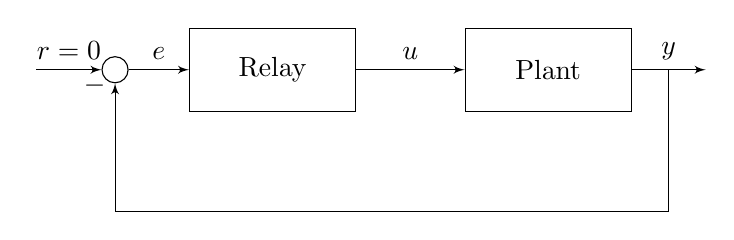
\begin{tikzpicture}[auto, node distance=2cm,>=latex']
    % We start by placing the blocks
    \node [input, name=input] {};
    \node [sum, right of=input] (sum) {};
    \node [block, right of=sum] (relay) {Relay};
    \node [block, right of=relay, node distance = 3.5cm] (plant) {Plant};
    % We draw an edge between the controller and system block to 
    % calculate the coordinate u. We need it to place the measurement block. 
    \draw [->] (relay) -- node[name=u] {$u$} (plant);
    \node [output, right of=plant] (output) {};
    \node [output, below of=u] (measurements) {Measurements};

    % Once the nodes are placed, connecting them is easy. 
    \draw [draw,->] (input) -- node {$r = 0$} (sum);
    \draw [->] (sum) -- node {$e$} (relay);
    \draw [->] (plant) -- node [name=y] {$y$}(output);
    \draw [-] (y) |- (measurements);
    \draw [->] (measurements) -| node[pos=0.99] {$-$} 
        node [near end] {} (sum);
\end{tikzpicture}
\end{center}
\end{frame}

\subsection{Motivation}
\begin{frame}
\frametitle{Motivation}
\begin{itemize}
\item Historically classical field
\item Auto-tuning of process controllers
\item Simplify biological oscillations
\item Unsolved research problems exist
	\begin{itemize}
	\item Why do the oscillations converge towards the limit cycle so quickly?
	\item Is it possible to have several limit cycles depending on the initial conditions?
 \end{itemize}
\end{itemize}
\end{frame}


\subsection{Theory}
\begin{frame}
\frametitle{Theory}
\framesubtitle{K.J.\r{A}str\"{o}m, \emph{Oscillations in systems with relay feedback}, (1995)}
\begin{columns}[t,onlytextwidth]
\column{.75\textwidth}
	\begin{itemize}
    \item Conditions for limit cycles
    \item Conditions for local stability
	\item Initial conditions for oscillations
  \end{itemize}
\column{.25\textwidth}
%\begin{center}
\begin{eqnarray*}
\dot{x} = Ax + Bu \\
y = Cx 
\end{eqnarray*}

%\end{center}
\end{columns}
\end{frame}

\section{FitzHugh-Nagumo}
\subsection{Intro}
\begin{frame}
\frametitle{FitzHugh-Nagumo model for action potentials}
\begin{columns}
\column{0.6\textwidth}
\begin{itemize}
\item Action potential % Short lasting event where electrical membrane potential of a nerve cell rapidly rises and falls.
\item Hodgkin-Huxley model % Developed a model to describe the action potential. The key idea was the use of voltage and time dependent conductances of various ion channels. Noble Prize in Physiology or Medecine 1952
\begin{itemize}
\item Four variables
\item Fast and slow variables
\end{itemize}
\item FitzHugh-Nagumo model extracts the essential behaviour
\item Only two variables
\end{itemize}
\column{.4\textwidth}
\begin{figure}
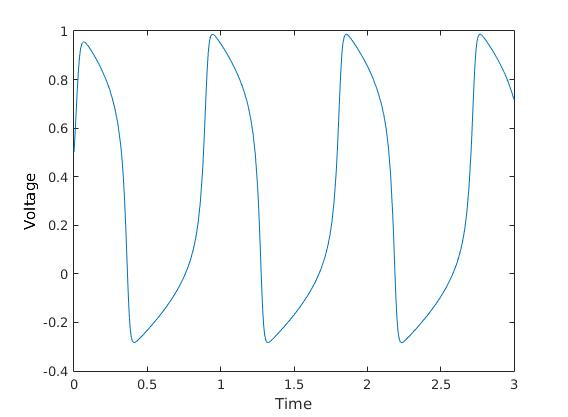
\includegraphics[width = \textwidth]{AP_fitz_nagumo}
\end{figure}
\end{columns}
\end{frame}

\subsection{Speed of fast variable}
\begin{frame}
\frametitle{FitzHugh-Nagumo}
	\begin{align*}
	\epsilon\frac{dv}{dt} &= f(v) - i + I_{\text{app}} \\
	\frac{di}{dt} &= v - \gamma i\\
	\end{align*}
	\vspace{-1cm}
	\begin{columns}
		\column{.5\textwidth}
		\begin{figure}
		        \includegraphics<1>[width=\textwidth]{fitz_nagumo_voltage_time}
				\includegraphics<2>[width=\textwidth]{fitz_nagumo_speed_voltage_time}
		\end{figure}
		
		\column{.5\textwidth}
		\begin{figure}
		        \includegraphics<1>[width=\textwidth]{fitz_nagumo_hysteresis.png}
				\includegraphics<2>[width=\textwidth]{fitz_nagumo_speed}
		\end{figure}
	\end{columns}
\end{frame}

\subsection{Modelling using relay feedback}
\begin{frame}
\frametitle{FitzHugh-Nagumo and Relay feedback}
\begin{columns}
\column{0.5\textwidth}
\begin{figure}
		        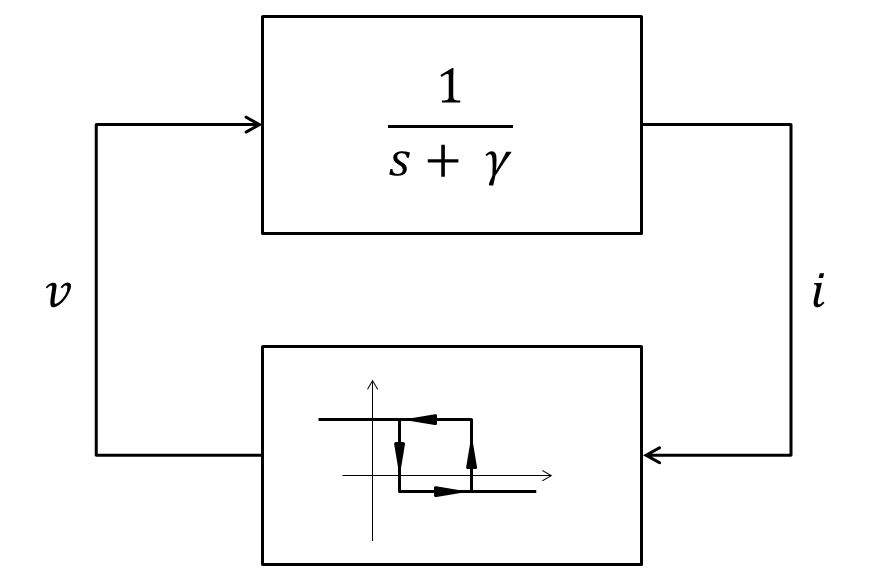
\includegraphics[width=\textwidth]{fitz_relay_transfer}
\end{figure}
\column{0.5\textwidth}
\begin{figure}
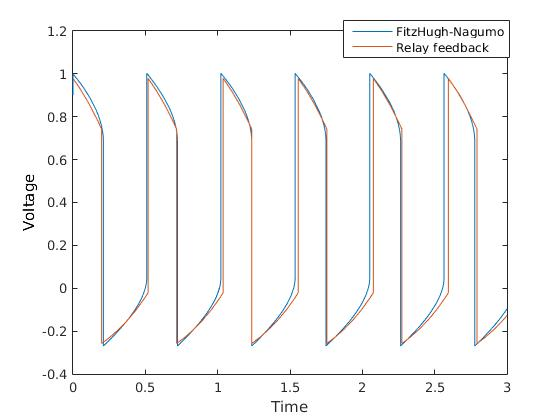
\includegraphics[width = \textwidth]{fitz_rot_relay_voltage_time}
\end{figure}
\end{columns}
\end{frame}


\section{Goodwin Oscillator}
\subsection{Intro}
\begin{frame}
	\frametitle{Goodwin Oscillator}
	
	\begin{itemize}
	\item Biochemical oscillator based on negative feedback
	\item Concentration of mRNA, protein and end product
	\end{itemize}
	

	\begin{align*}
	\text{mRNA \hspace{1cm}}\frac{dx_1}{dt'} &= \frac{1}{1 + x_3^p} - b_1x_1 \\
	\text{Protein \hspace{1cm}}	\frac{dx_2}{dt'} &= b_2(x_1 - x_2) \\
	\text{Product \hspace{1cm}}	\frac{dx_3}{dt'} &= b_3(x_2 - x_3) \\
	\end{align*}

%	\begin{figure}
%	\includegraphics<2>\\[width=0.7\textwidth]{goodwin_nonlinear_element}
%	\end{figure}
\end{frame}

\begin{frame}
\frametitle{Goodwin Oscillator}
\begin{figure}
	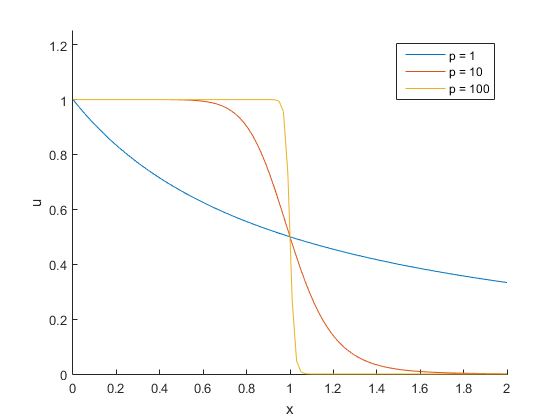
\includegraphics[width=0.7\textwidth]{goodwin_nonlinear_element}
\end{figure}
\end{frame}

\subsection{Modelling with relay feedback}
\begin{frame}
\frametitle{Goodwin Oscillator and Relay Feedback}
\begin{columns}
\column{0.5\textwidth}
\begin{figure}
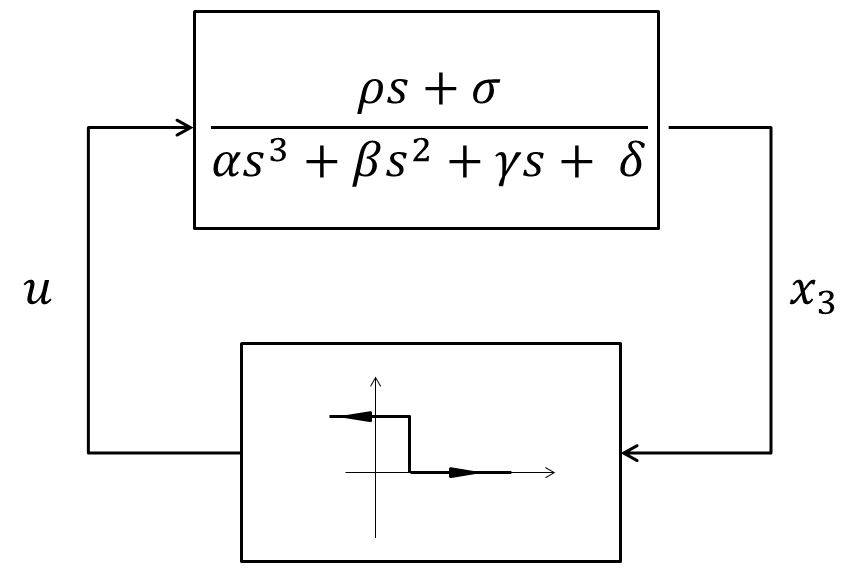
\includegraphics[width=\textwidth]{goodwin_relay_transfer}
\end{figure}
\column{0.5\textwidth}
\begin{figure}
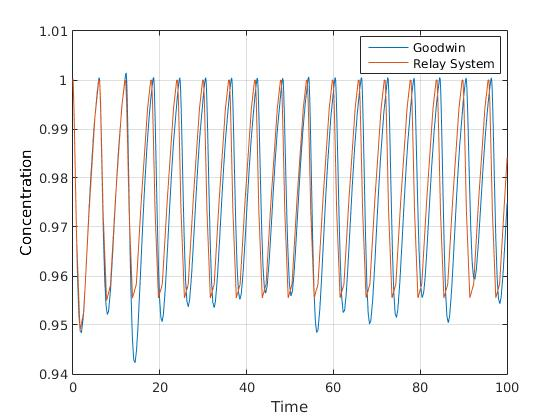
\includegraphics[width=\textwidth]{goodwin_relay_x3}
\end{figure}
\end{columns}
\end{frame}


\section{Conclusions}
\subsection{Future work}
\begin{frame}
\frametitle{Next Term}
\begin{itemize}
\item Study differential positivity and its application to relay feedback
\item Apply this analysis tool to biological oscillations approximated by relay feedback 
\end{itemize}
\end{frame}

\subsection{Conclusion}
\begin{frame}
\frametitle{Conclusions}
	\begin{itemize}
	\item Studied oscillations of relay feedback systems
    \item Bridged classical control theory with non-linear oscillations currently being studied in biology
    \begin{itemize}
	\item FitzHugh-Nagumo model 
    \item Goodwin Oscillator model
\end{itemize}
	\item Study differential positivity
	\item Apply this analysis to relay feedback systems
	\end{itemize}
\end{frame}



\end{document}